\subsubsection{Recirculation algorithm}
%TODO image of the algorithm 
%TODO shorten the text 

TODO spomenut ze unsupervised 

We will outline the main ideas used for this Recirculation algorithm. They motivation is in an autoencoder (or data-compression) and they also mention the PCA algorithm. 

First, there are just two layers - visible and hidden which are connected by directed weights (most of time we assume these weights as symmetric). 

Second, we operate in discrete time. Each learning phase has four steps. In first two the input is propagated to hidden layer. In second two the desired output is propagated to hidden layer. The learning on visible layer occurs in second step when the desired output meets the reconstructed input. Similary, the learning on hidden layer occurs in step 3.

Third, the learning rules for both layers is almost identical (we can non-formally write that they are symmetric). It is interesting that the learning rule uses no exact ifnormation about the non-linear function (usually logistics), but only assumes that it has bounded derivate. The learning rule is an approximation of the learning rule derived from the difference equations for error correction. 

Authors study the case of asymetric weights. They do not provide a proof of convergence but they provide some intutition why it should work. Also they link the work of Ballard who experimented with connecting (merging) several closed loops so that hidden units of closed loops can be input units of other closed loops of recirculation.

\paragraph{From the original article.}
Instead of using a separate group of units for the input and output we use the very same group of \textit{visible} units, so the input vector is the initial state of this group and the output vector is the state after information has passed around the loop. The difference between the activity of a visible unit before and after sending activity around the loop is the derivative of the squared reconstruction error \citet{hinton1988learning}.

On the first pass, the original visible vector is passed around the loop, and on the second pass ana average of the original vector and the reconstructed vector is passed around the loop. The learning procedure changes each weight by an amount proportional to the product of the \textit{presynaptic} activity and the \textit{difference} in the post-synaptic activity on the two passes  \citet{hinton1988learning}.

$$\Delta w_{ij} = \epsilon y_j(1)[y_i(0)-y_i(2)],$$
$$\Delta w_{ji} = \epsilon y_i(2)[y_j(1)-y_j(3)],$$
where $y_i(t)$ is the activation value of unit $i$ in time $t$.

With approximation we can derive the following learning rule
$$\frac{\partial E}{\partial w_{ji}} \approx \frac{1}{1-\lambda}y_i(2)[y_j(3)-y_j(1)].$$
An interesting property of this equation is that it does not contain a term for the gradient\footnote{We assume that it is differentiable, it is monotonous and has bounded derivate.} of the input-output function of unit $j$ so recirculation learning can be applied even when unit $j$ uses an unknown non-linearity \citet{hinton1988learning}. 

%TODO: Understand why exactly we assume the linearity of the visible layer.

%TODO: Go through the derivation of the learning rule to understand why it is working as the gradient descent. 

\paragraph{O'Reillys conclusion.}

$$\frac{\partial E}{\partial h_j} = - (\sum_k t_k w_{jk} - \sum_k o_k w_{jk})$$
Thus, instead of having a separate error-backpropagation phase to communicate error signals, one can think in terms of standard activation propagation occuting via reciprocal (and symmetric) weights that come from the ouput units to the hidden units \citet{o1996bio}. 

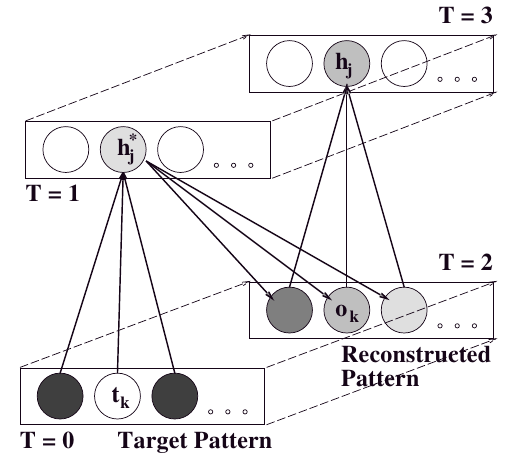
\includegraphics[width=15px]{img/recirculation.png}
